% Chapter 5. Experiments 1 to 7.
% Every number in this chapter comes from verify/registry.json (keys named in the
% text or caption), from the reaction list thermo/Networks/Nominal.txt, or from the
% figure manifests in figures/manifest/.

\chapter{Experiments 1 to 7}
\label{ch:exp17}

The first seven experiments ask what the absorber does inside the model, before any
candidate is tested. Experiments~1 and~2 switch it on, Experiment~3 tests whether its
effect scales with its amount, Experiments~4 to~6 locate the effect in wavelength, in
reaction and in altitude, and Experiment~7 moves the absorber up and down. Every
comparison follows the conventions of Chapter~\ref{ch:conv}. Unless stated otherwise,
each experiment compares the run with the absorber on ($A_{\mathrm{UUV}} = 1$) against
the control ($A_{\mathrm{UUV}} = 0$).

% ===========================================================================
\section{Experiments 1 and 2: does the absorber do anything?}
\label{sec:e12}

\textbf{Experiment~1} ran the model with the absorber term present but its amplitude set
to zero, and compared the result with a second run of the unchanged model, made on the project
computer before the term was switched on (keys beginning \texttt{e1.ref}; it is a separate
run from the baseline of Section~\ref{sec:baseline}). The two should differ only by run-to-run scatter, and they do: the mean
relative change in actinic flux, taken over every element of the field
(Section~\ref{sec:conv-mean}), is 0.013553\% (\texttt{e1.aflux.meanrel}), and in both
runs the solver's own budget of every chemical element closes to better than one part in
ten thousand (keys \texttt{e1.A0.atom\_loss} and \texttt{e2.A1.atom\_loss}). The control
is therefore the model as supplied.

\textbf{Experiment~2} switched the absorber on. Figure~\ref{fig:F5} shows what it does.
The absorber adds optical depth in and above the clouds, and the radiation field changes
mainly between 300 and 420~nm and between 69 and 93~km. The largest single change in
actinic flux is $-4.6982\times10^{12}$ photons per square centimetre per second per
nanometre, at 81~km and 328~nm (\texttt{e2.aflux.delta\_at\_arg}), a fall from
$7.2246\times10^{13}$ to $6.7548\times10^{13}$. Over all lit elements of the field the
mean relative change is 3.7078\% and the largest is 87.404\%
(\texttt{e3fp.bnd.A1.aflux.mean\_pct} and \texttt{.max\_pct}).

\begin{figure}[tbp]
  \centering
  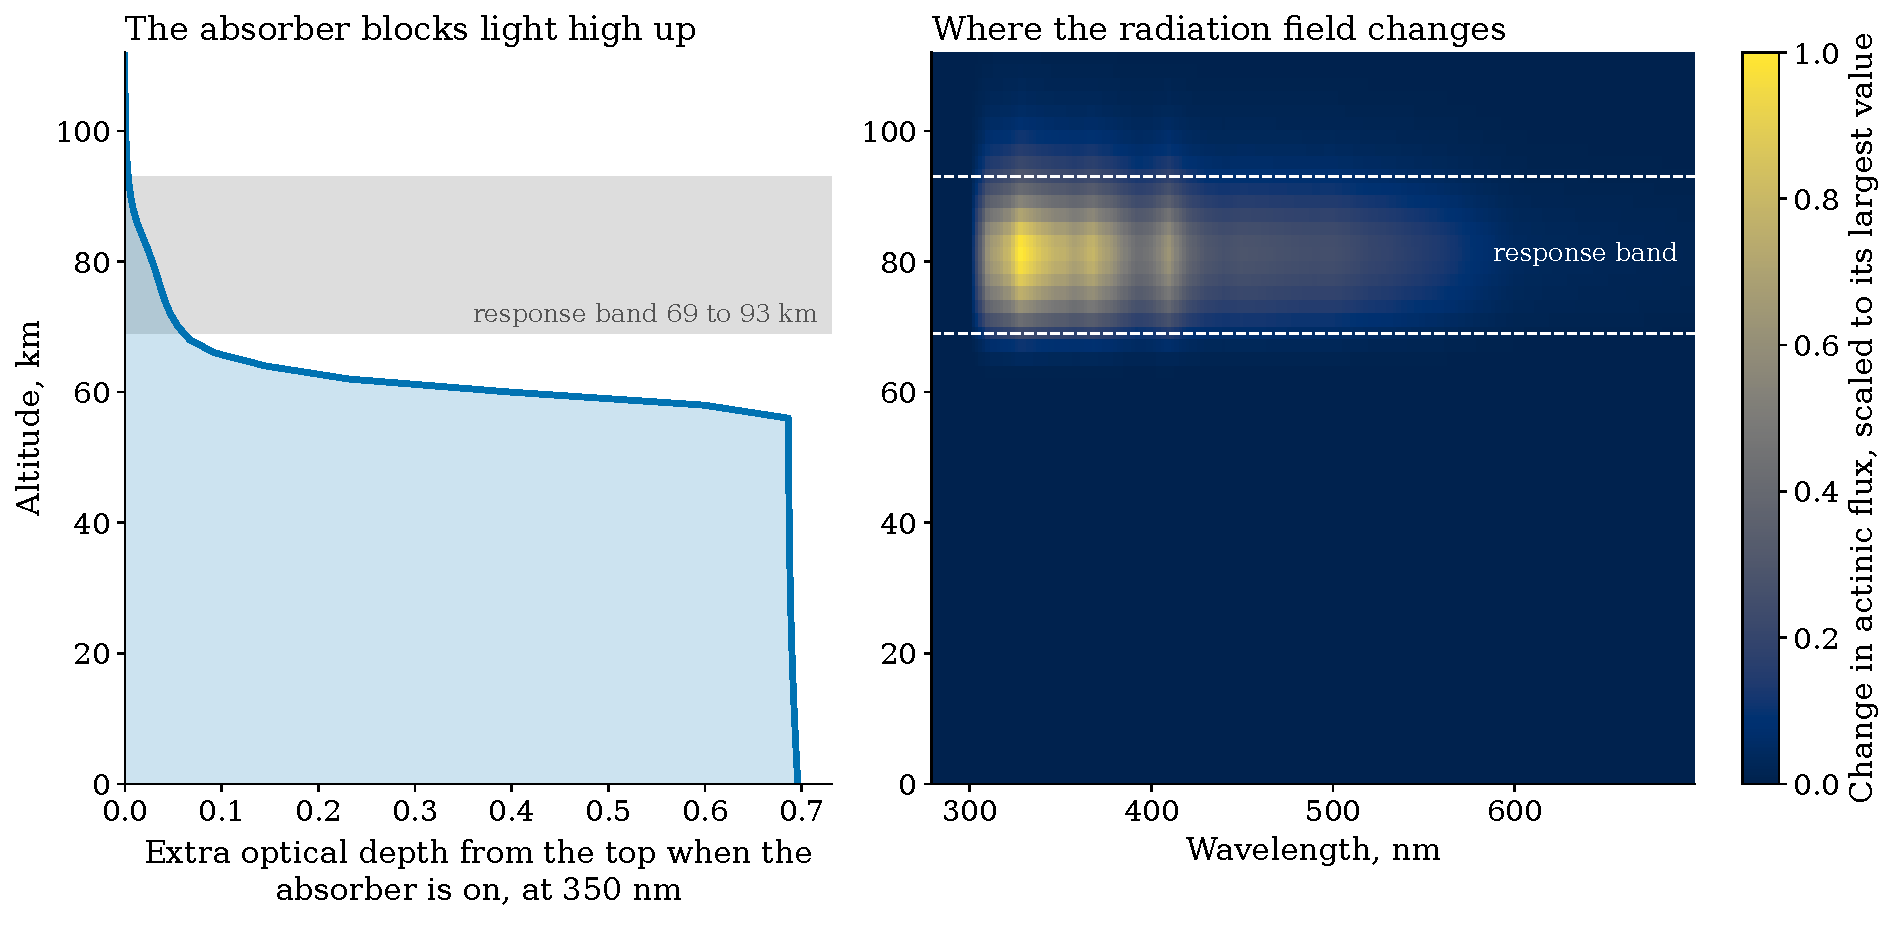
\includegraphics[width=\textwidth]{F05_E01-02_absorber-effect_ch5_s7.pdf}
  \caption[What the absorber does when it is switched on (Experiments~1 and~2)]{What the absorber does when it is switched on (Experiments~1 and~2). Left:
    the extra optical depth, counted from the top of the atmosphere, that the absorber
    adds at 350~nm. Right: the change in actinic flux, scaled to its largest value; it
    sits between 69 and 93~km and mostly between 300 and 420~nm. Sources: committed output of
    Experiments~1 and~2; registry keys \texttt{e6.interval.90.lo} and \texttt{.hi}.}
  \label{fig:F5}
\end{figure}

The composition responds far less. The largest change in the SO\sub{2} mixing ratio is
0.2243\%, and in SO 1.7399\%, both at 71~km (\texttt{e2.SO2.maxrel} and
\texttt{e2.SO.maxrel}). Both are smaller than the reproducibility floor of
Section~\ref{sec:conv-floor}, so they are upper bounds. A strong change in radiation
that leaves the main sulfur species almost unmoved is the pattern that every later
experiment had to explain, and it is why the response was next traced in amount,
wavelength, reaction and altitude.

% ===========================================================================
\section{Experiment 3: is the response proportional?}
\label{sec:e3}

If the response grows in proportion to the amount of absorber, a result found at one
amount holds at any other, and later experiments can compare candidates of different
strength fairly. Besides the control (amplitude 0, run A0) and the nominal run of
Experiment~2 (amplitude 1, run A1), Experiment~3 added two runs, A0.5 at half and A2 at
twice the nominal amplitude.

The test compares the change at half amplitude with half the change at full amplitude,
element by element; a ratio of exactly 1 means proportional. Over the absorber's own
wavelength range, 300 to 698~nm, the median ratio is 1.00002 for optical depth and
1.00208 for actinic flux. Outside that range the two runs differ from the control only
by round-off, thousands of times smaller than the real changes inside it, so a ratio
there carries no information. A second test, on the whole actinic flux field at once,
gives 1.010795 at half amplitude and 0.979304 at twice the amplitude.
Figure~\ref{fig:F6} shows the result.

{\raggedright The keys for these numbers, in order, are
\texttt{e3.\allowbreak lin.\allowbreak tau.\allowbreak inband.\allowbreak median}, \texttt{e3.\allowbreak lin.\allowbreak aflux.\allowbreak inband.\allowbreak median},
\texttt{e3fp.\allowbreak aflux.\allowbreak ratio.\allowbreak A0p5} and \texttt{e3fp.\allowbreak aflux.\allowbreak ratio.\allowbreak A2p0}; the round-off
comparison is \texttt{e3.lin.tau.\allowbreak outband.\allowbreak median\_relsize} against
\texttt{e3.lin.tau.\allowbreak inband.\allowbreak median\_relsize}.\par}

\begin{figure}[tbp]
  \centering
  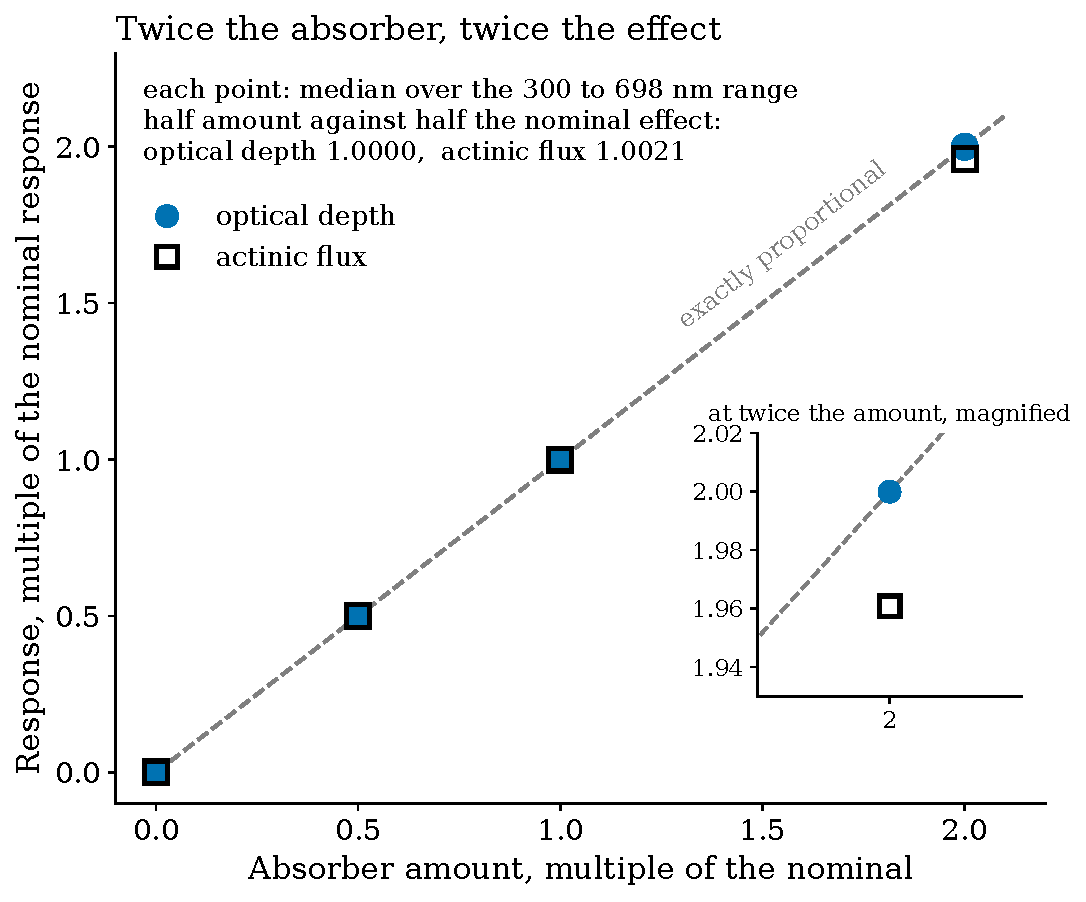
\includegraphics[width=0.6\textwidth]{F06_E03_linear-response_ch5_s8.pdf}
  \caption[The radiative response is proportional to the amount of absorber (Experiment~3)]{The radiative response is proportional to the amount of absorber
    (Experiment~3). Each point is the response at that amount as a multiple of the
    response at the nominal amount. Registry keys \texttt{e3.lin.tau.inband.median} and
    \texttt{e3.lin.aflux.inband.median}.}
  \label{fig:F6}
\end{figure}

The radiative response is therefore proportional to the amount of absorber across a
factor of four. The same test on the sulfur reservoirs gives ratios far from 1 at half
amplitude: for SO\sub{2} it is 1.916 (\texttt{e3fp.L2.A0p5.SO2.ratio}). This
could be read as a sign that the chemistry responds non-proportionally, but that
reading cannot be supported. The SO\sub{2} and SO\sub{3} changes are below the
reproducibility floor: two runs that the radiation cannot tell apart differ in their
reservoirs by about as much (Section~\ref{sec:conv-floor}). SO alone goes above it, at
most 3.316\% at half and 4.379\% at twice the amplitude, inside the band at 71~km
(\texttt{e3fp.A0p5.SO.maxrel\_pct} and \texttt{e3fp.A2.SO.maxrel\_pct}); since the floor
is the smallest the scatter can be (Section~\ref{sec:conv-floor}), that margin is too
narrow to settle the question. The radiative result stands; the chemical one is not
resolved.

% ===========================================================================
\section{Experiment 4: which wavelengths?}
\label{sec:e4}

Experiment~4 asked where in wavelength the response comes from, in two stages.

\textbf{Stage 4A} took the control and the nominal run (A0 and A1) and split each photolysis rate change at
81~km, the middle of the response, into the wavelength windows it came from, using VULCAN's own rule
(Section~\ref{sec:conv-quad}). Different molecules draw on different parts of the
spectrum. S\sub{2}O takes 93.689\% of its change from 300 to 320~nm
(\texttt{e4a.S2O\_1.300\_320.pct}); S\sub{3} takes 49.605\% from 380 to 420~nm; S\sub{4}
takes all of it from beyond 420~nm. SO\sub{2} itself takes none of its change from these
windows, because in the model it is broken apart only by light shorter than 225~nm
(its photolysis cross section, \texttt{cross\_J}, is zero above that). Its photolysis
therefore changes only indirectly, a point Experiment~7 confirms.

Table~\ref{tab:e4a} gives the split for ten sulfur and chlorine photolysis branches,
ordered from the shortest wavelengths to the longest. S\sub{2}O and SO\sub{3} take
nearly all of their change from below 340~nm; S\sub{3}, ClS\sub{2} and SCl take most of
theirs above 380~nm; OSSO, SCl\sub{2} and Cl\sub{2} draw on the whole range. A candidate
that absorbs at some wavelengths therefore affects the photolysis of some molecules and
not others, and which molecules depends on where its absorption lies.

\begin{table}[htbp]
  \centering
  \caption[Where in wavelength each photolysis change comes from (Experiment~4, Stage~4A)]{Where in wavelength the change in each photolysis rate coefficient comes from,
    when the absorber is switched on (Experiment~4, Stage~4A), at 81~km, in per cent of the
    change.
    Ten sulfur and chlorine branches; keys \texttt{e4a.<branch>.<window>.pct}. A row can
    fall short of 100 by the small part from outside these windows.}
  \label{tab:e4a}
  \footnotesize
  \setstretch{1.0}
  \begin{tabular}{lcccccc}
    \toprule
    & \multicolumn{6}{c}{Window (nm)} \\
    \cmidrule(lr){2-7}
    Branch & 300 to 320 & 320 to 340 & 340 to 360 & 360 to 380 & 380 to 420 & 420 to 620 \\
    \midrule
    S\sub{2}O & 93.689 & 6.299 & 0 & 0 & 0 & 0 \\
    SO\sub{3} & 80.754 & 18.795 & 0 & 0 & 0 & 0 \\
    S\sub{2}Cl\sub{2} & 45.016 & 43.215 & 8.574 & 2.872 & 0.319 & 0 \\
    Cl\sub{2} & 17.513 & 40.010 & 25.976 & 11.616 & 4.207 & 0.679 \\
    OSSO (S\sub{2}O\sub{2}) & 13.535 & 25.173 & 21.336 & 19.184 & 14.786 & 5.985 \\
    SCl\sub{2} & 11.427 & 29.895 & 23.971 & 15.863 & 15.974 & 2.869 \\
    S\sub{3} & 0 & 0 & 7.858 & 30.566 & 49.605 & 11.970 \\
    ClS\sub{2} & 0 & 5.785 & 15.369 & 26.717 & 40.776 & 11.353 \\
    SCl & 0 & 0.669 & 5.392 & 10.102 & 31.024 & 52.812 \\
    S\sub{4} & 0 & 0 & 0 & 0 & 0 & 100 \\
    \bottomrule
  \end{tabular}
\end{table}

\textbf{Stage 4B} tested this with six new runs, B1 to B6, each with the absorber spectrum
kept only inside one window: 300 to 320, 320 to 340, 340 to 360, 360 to 380, 380 to 420
and 420 to 698~nm, in that order. Figure~\ref{fig:F7} shows that each run changes the radiation field only where
its absorber absorbs; outside its window the change is too small to see at this scale.
The response is \emph{spectrally local}: what the absorber does at one wavelength does not
depend on what it does at another. This is what makes a test of spectral shape
meaningful in Experiment~12. The six runs also share one response altitude, which
Section~\ref{sec:conv-band} used to show that the response band belongs to the
atmosphere, not to the spectrum.

\begin{figure}[tbp]
  \centering
  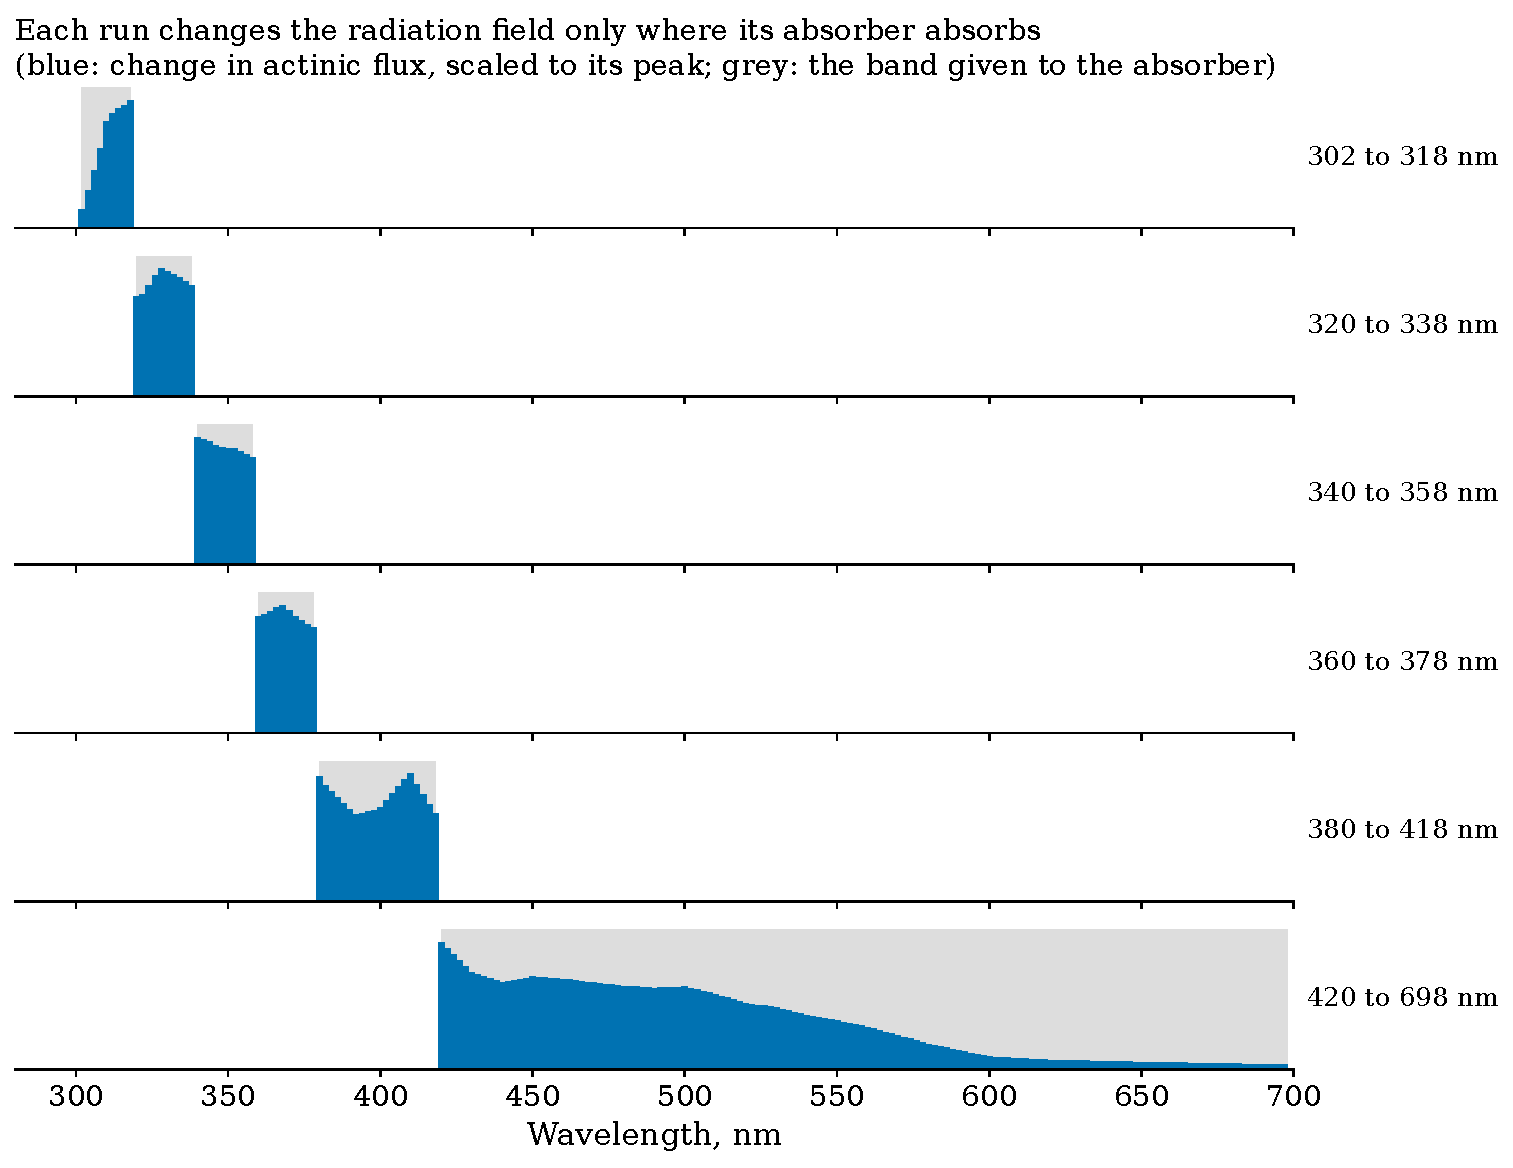
\includegraphics[width=0.82\textwidth]{F07_E04_spectrally-local_ch5_s9.pdf}
  \caption[Each band-limited run changes the radiation field only inside its own window (Experiment~4, Stage 4B)]{Each band-limited run changes the radiation field only inside its own window
    (Experiment~4, Stage 4B). Blue: change in actinic flux, scaled to its peak. Grey: the
    wavelengths given to the absorber in that run. Registry keys
    \texttt{e4b.<run>.support\_lo} and \texttt{.support\_hi}.}
  \label{fig:F7}
\end{figure}

% ===========================================================================
\section{Experiment 5: which reactions?}
\label{sec:e5}

VULCAN writes its chemistry as program code: the rate of change of each species is a
long sum of signed terms, one for each reaction that makes or destroys it. For SO\sub{2}
the sum has 63 terms from 58 distinct reactions (\texttt{e5.SO2.nterms} and
\texttt{.nunique}). Experiment~5 read these terms out of the generated file
\texttt{chem\_funs.py} and evaluated each one in both runs. Adding the terms back
together gives the model's own rate of change exactly, with zero error, for all five
sulfur species examined and in both runs (keys ending \texttt{extraction\_error}). The
attribution is therefore the model's own arithmetic.

\begin{figure}[tbp]
  \centering
  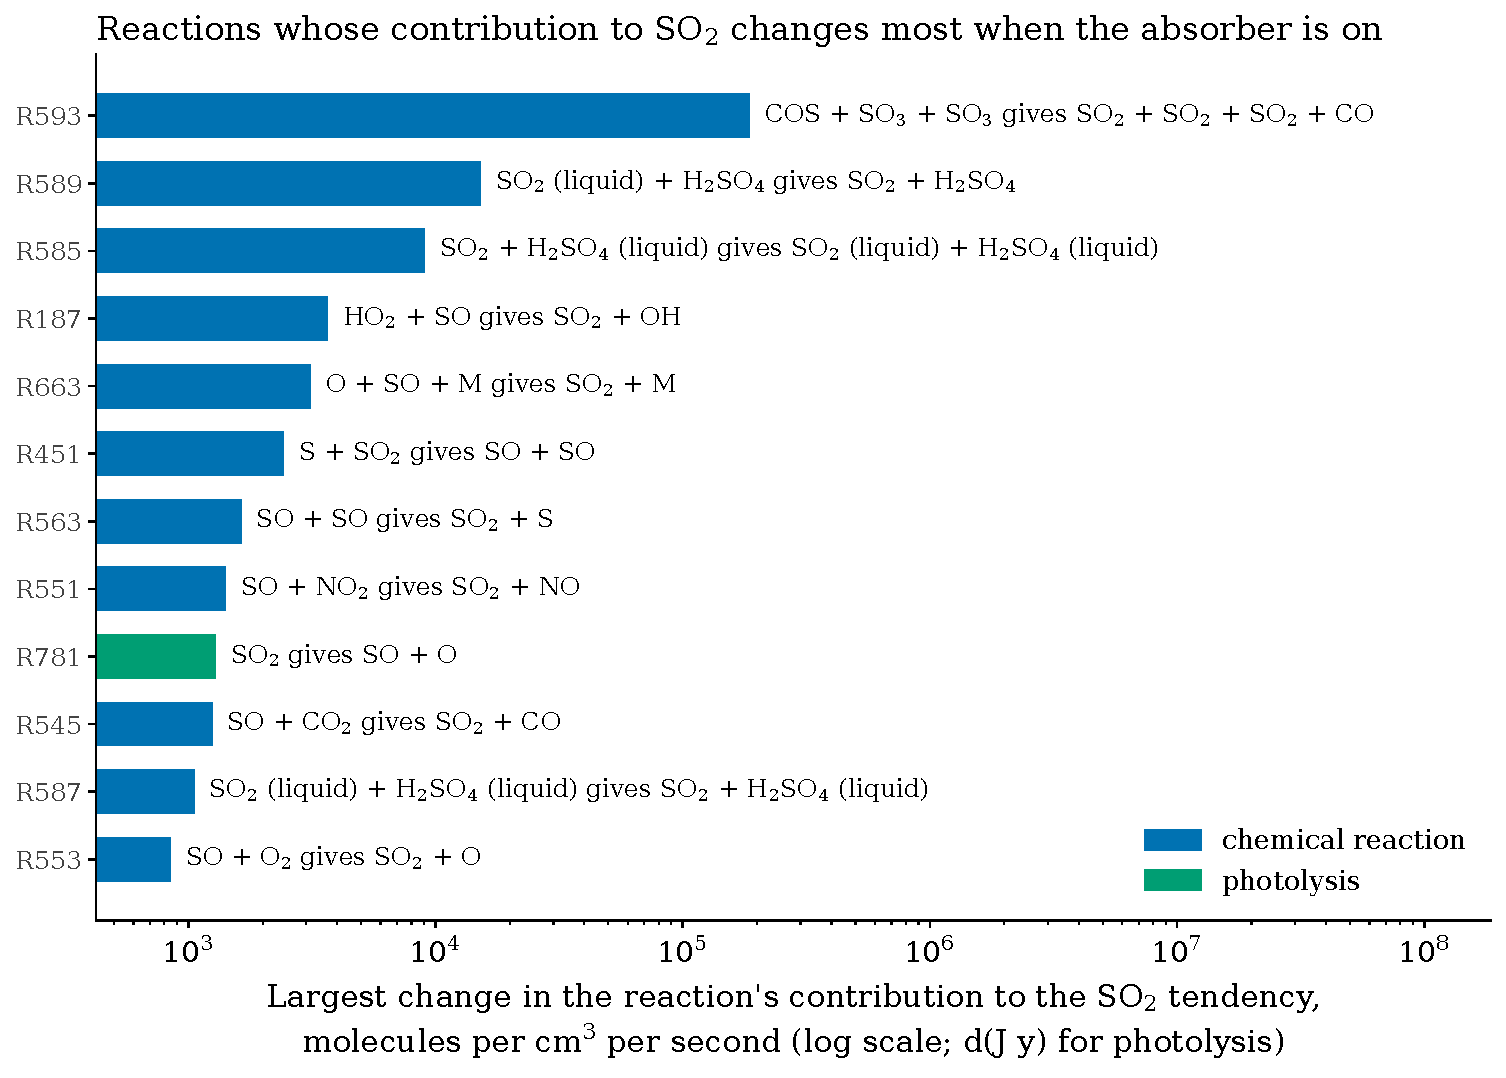
\includegraphics[width=0.86\textwidth]{F08_E05_reaction-pathways_ch5_report.pdf}
  \caption[The reactions whose contribution to SO\sub{2} changes most (Experiment~5)]{The reactions whose contribution to SO\sub{2} changes most when the absorber is
    switched on (Experiment~5), on a logarithmic scale. For the photolysis R781 the
    quantity is the change in rate, $\Delta(Jn)$, written d(J y) on the axis because the
    model calls the number density y. Source: registry keys
    \texttt{e5.SO2.<reaction>.maxdelta}; reaction labels from
    \texttt{thermo/Networks/Nominal.txt}.}
  \label{fig:F8}
\end{figure}

Figure~\ref{fig:F8} ranks the reactions by how much their contribution to SO\sub{2}
changes. The largest change is in R593, COS + SO\sub{3} + SO\sub{3} $\rightarrow$
3\,SO\sub{2} + CO, at $1.8644\times10^{5}$ molecules per cubic centimetre per second at
35~km (\texttt{e5.SO2.R593.maxdelta}). But that reaction runs at $5.7568\times10^{8}$
there (\texttt{e5.SO2.R593.bg\_A0}), so it changes by only 0.032385\%. The oxidation
O + SO + M $\rightarrow$ SO\sub{2} + M (R663) changes by far less in absolute terms but by
1.3809\% of its own rate, at 71~km (\texttt{e5.SO2.R663.frac\_pct}). The absorber reaches
the sulfur chemistry through several coupled reactions, not one, and the largest
absolute change does not mark the most affected reaction. Changes of this size in
reaction rates that depend on abundances also sit below the reproducibility floor, so
the experiment shows \emph{where} the response enters the chemistry more reliably than
\emph{how much}.

% ===========================================================================
\section{Experiment 6: which altitudes?}
\label{sec:e6}

Experiment~6 located the response in altitude. Its radiative part defines the response
band, 69 to 93~km, set out in Section~\ref{sec:conv-band}; Figure~\ref{fig:F9} shows the
profile. The experiment also located the reactions, using the change in rate,
$\Delta(Jn)$ (Section~\ref{sec:conv-J}). The photolysis reactions that the absorber acts
on directly sit in the same band. Of the change in SO\sub{2} photolysis (R781), 99.128\%
falls between 69 and 93~km, with its peak at 71~km (\texttt{e6.R781.pct\_in\_band} and
\texttt{.peak\_z}); for SO\sub{3} photolysis (R787) the share is 99.992\%, peaking at
73~km. Some large changes in other reactions lie much lower: R593 peaks at 35~km and R589
at 53~km, with almost nothing in the band. These are knock-on effects carried through the
chemistry and by mixing, not direct effects of the absorber on sunlight.

\begin{figure}[tbp]
  \centering
  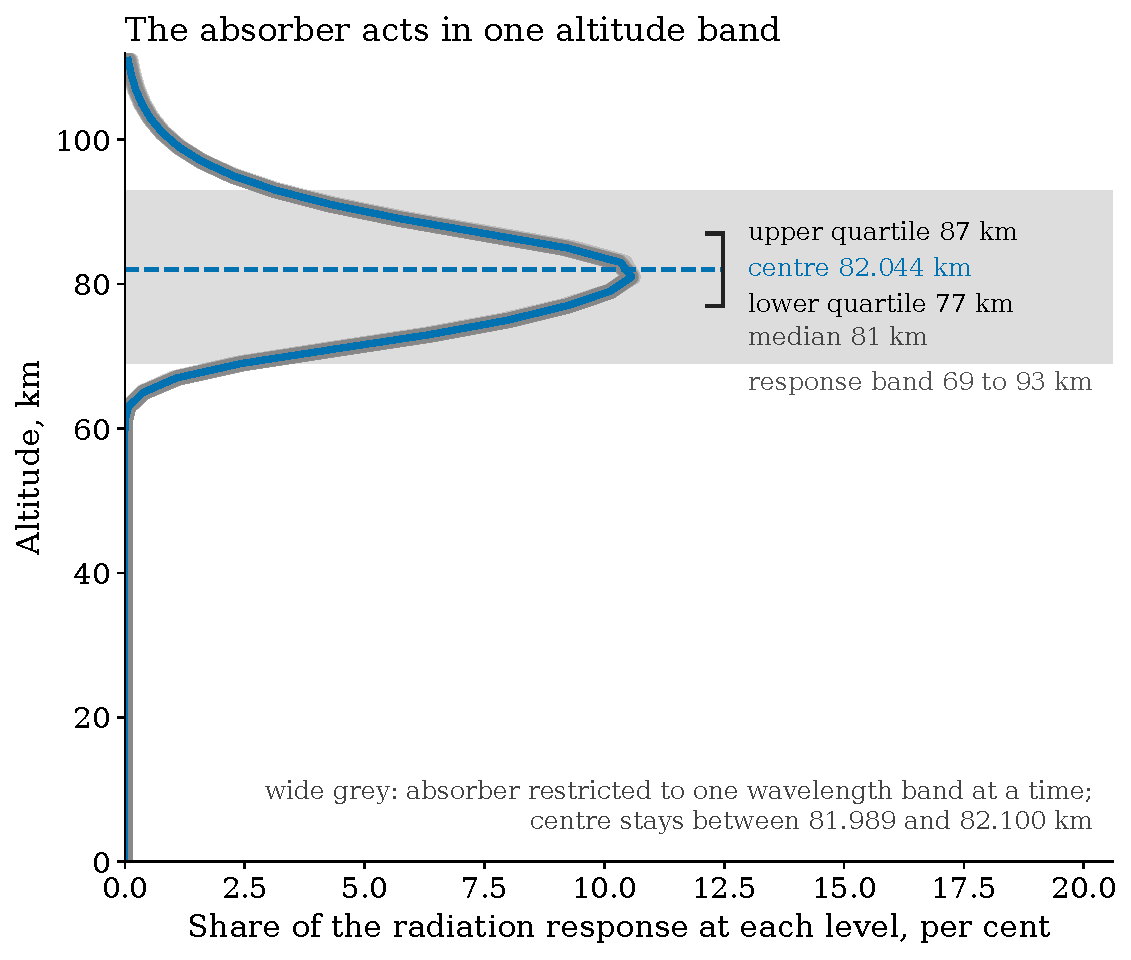
\includegraphics[width=0.6\textwidth]{F09_E06_response-band_ch5_s10.pdf}
  \caption[The share of the radiative response at each altitude (Experiment~6)]{The share of the radiative response at each altitude (Experiment~6). Blue: the
    full absorber. Wide grey lines: the six band-limited runs of Experiment~4. Registry
    keys \texttt{e6.A1.meanz}, \texttt{e6.A1.q25}, \texttt{.q50}, \texttt{.q75},
    \texttt{e6.interval.90.lo} and \texttt{.hi}, \texttt{e6.B5.meanz} and
    \texttt{e6.B6.meanz}.}
  \label{fig:F9}
\end{figure}

% ===========================================================================
\section{Experiment 7: does it matter where the absorber sits?}
\label{sec:e7}

Experiment~7 moved the whole absorber profile up in one run (Experiment~7A) and down in
another (7B), keeping the spectrum, the
amplitude and the total number of particles fixed at $4.0776\times10^{8}$ per square
centimetre (\texttt{e7.nominal.column}). Only the height changed. Its effect is measured
by $\Delta F$ of Equation~\eqref{eq:field}, the size of the change in the whole actinic
flux field as a percentage of the field with the absorber in its usual place.

The nominal profile is centred at 63.419~km (\texttt{e7.nominal.centroid}). Moving it
down by 18~km gives a centre of 45.419~km, a shift of exactly $-18.0000$~km. Moving it
up by 18~km gives 81.263~km, a shift of only $+17.8439$~km (registry key
\texttt{e7.7a.centroid\_shift}), because the top of the profile runs off the top of the
model and the rest is rescaled to keep the total fixed. The two moves are therefore not
mirror images, and the shift must not be written as $\pm 17.844$~km.

\begin{figure}[tbp]
  \centering
  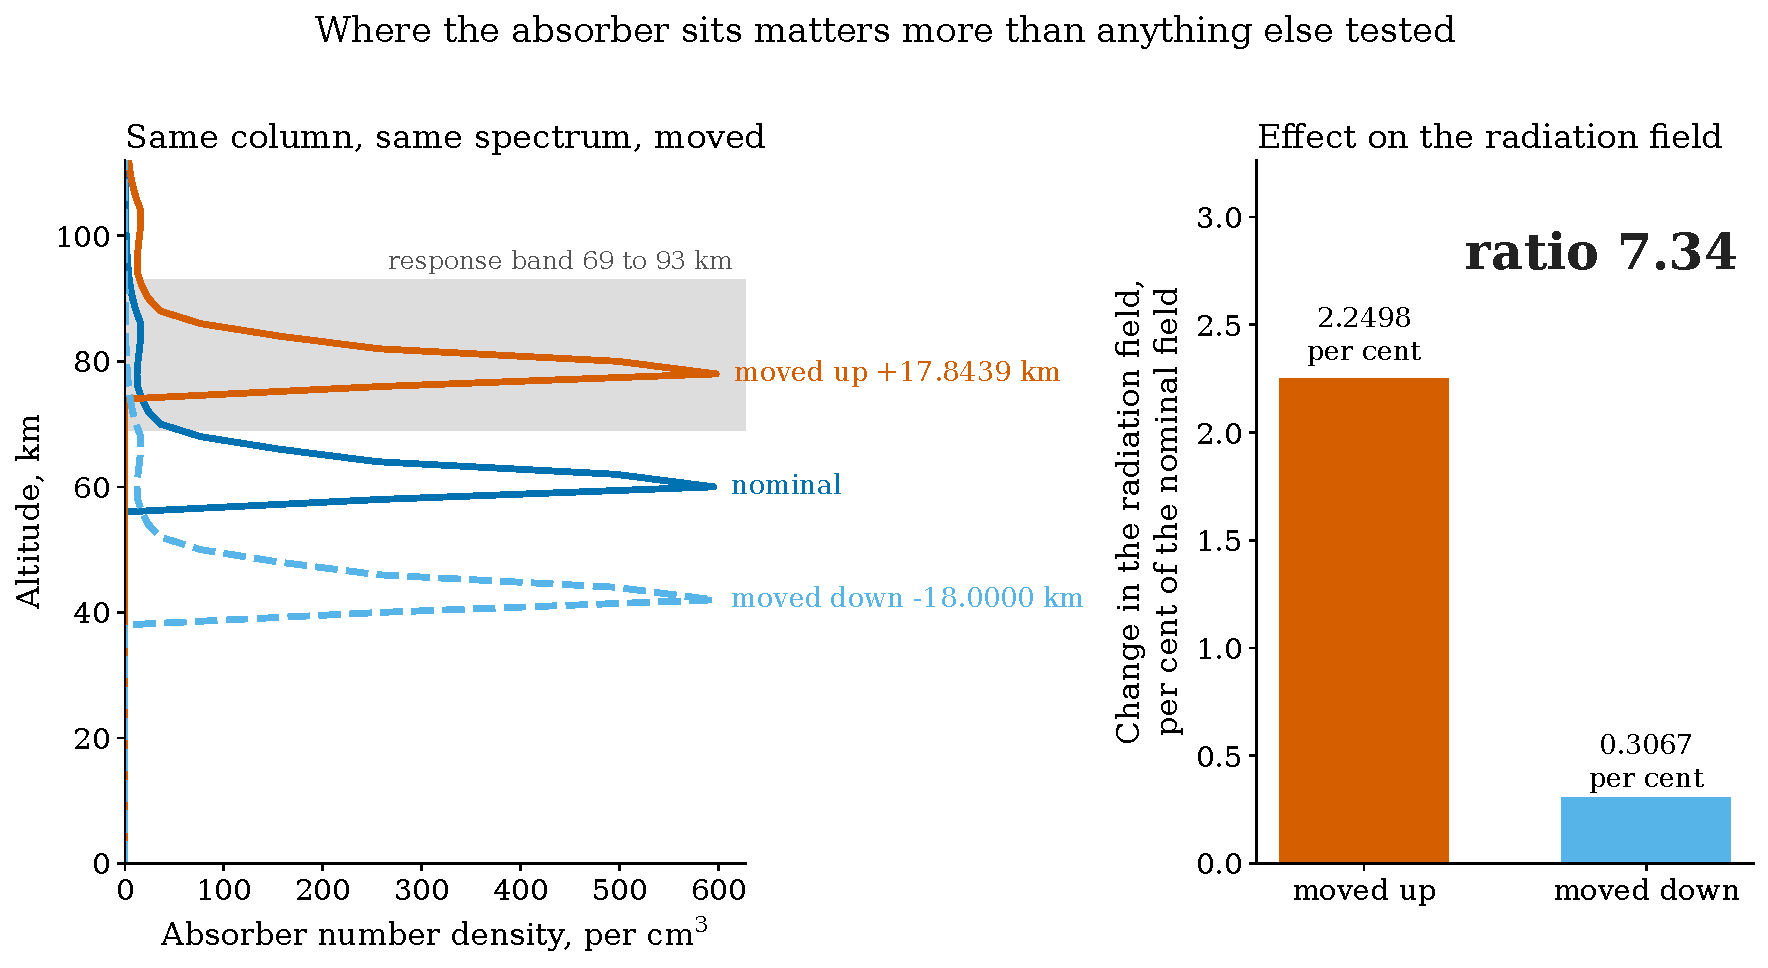
\includegraphics[width=\textwidth]{F10_E07_placement-first-order_ch5_s11.pdf}
  \caption[The same absorber, moved up or down, changes the radiation field by very different amounts (Experiment~7)]{The same absorber, moved up or down, changes the radiation field by very
    different amounts (Experiment~7). Left: the three absorber profiles, with the same
    total. Right: the change in the radiation field as a percentage of the nominal field.
    Registry keys \texttt{e7.7a.centroid\_shift}, \texttt{e7.7b.centroid\_shift},
    \texttt{e7a.L2pct}, \texttt{e7b.L2pct} and \texttt{e7.ratio\_7A\_over\_7B}.}
  \label{fig:F10}
\end{figure}

Figure~\ref{fig:F10} shows the result. Moved up, the absorber changes the radiation field
by 2.2498\% (\texttt{e7a.L2pct}); moved down, by 0.3067\% (\texttt{e7b.L2pct}). The same
amount of the same absorber has 7.34 times more effect when it sits higher
(\texttt{e7.ratio\_7A\_over\_7B}). The responding layer itself barely moves: the response
is centred at 82.435~km in the upward case and 82.355~km in the downward case
(\texttt{e7a.meanalt} and \texttt{e7b.meanalt}), close to the 82.044~km of
Experiment~6. An absorber high up overlaps that layer; the same absorber low down mostly
shades light that has already been weakened.

The chemistry confirms the picture. Three reactions whose rates are set by the local
light, R663, R551 (SO + NO\sub{2} $\rightarrow$ SO\sub{2} + NO) and R665 (O + SO\sub{2} + M
$\rightarrow$ SO\sub{3} + M), change in opposite directions when the absorber moves up
and when it moves down (keys \texttt{e7.7a} and \texttt{e7.7b} ending \texttt{.col}).
Three others, R187, R563 and R781, change in the same direction both ways; why is not yet
known, and it is recorded as an open question, not a result. Table~\ref{tab:e7rx} gives
the numbers: for each reaction, the change in its contribution to the SO\sub{2} budget,
added over the response band with the thickness in centimetres
(Section~\ref{sec:conv-col}). The upward move changes each of them several times more
than the downward move, as it changes the radiation field several times more.

\begin{table}[htbp]
  \centering
  \caption[Change in each reaction's contribution to the SO\sub{2} budget (Experiment~7)]{Change in each reaction's contribution to the SO\sub{2} budget, added over the
    response band, in molecules per square centimetre per second (Experiment~7). A
    positive value means the reaction adds more SO\sub{2} or removes less. Keys
    \texttt{e7.7a.SO2.<reaction>.col} and \texttt{e7.7b.SO2.<reaction>.col}.}
  \label{tab:e7rx}
  \footnotesize
  \setstretch{1.0}
  \begin{tabular}{lllr}
    \toprule
    Reaction & Equation & Moved up (7A) & Moved down (7B) \\
    \midrule
    R663 & O + SO + M $\rightarrow$ SO\sub{2} + M & $-5.6390\times10^{9}$ & $+6.6392\times10^{8}$ \\
    R551 & SO + NO\sub{2} $\rightarrow$ SO\sub{2} + NO & $+6.7343\times10^{9}$ & $-6.7855\times10^{8}$ \\
    R665 & O + SO\sub{2} + M $\rightarrow$ SO\sub{3} + M & $+3.1466\times10^{8}$ & $-6.1425\times10^{7}$ \\
    R187 & HO\sub{2} + SO $\rightarrow$ SO\sub{2} + OH & $-3.8755\times10^{9}$ & $-5.2023\times10^{8}$ \\
    R563 & SO + SO $\rightarrow$ SO\sub{2} + S & $+1.3783\times10^{9}$ & $+3.1740\times10^{8}$ \\
    R781 & SO\sub{2} + $h\nu$ $\rightarrow$ SO + O & $+8.2352\times10^{8}$ & $+2.2860\times10^{8}$ \\
    \bottomrule
  \end{tabular}
\end{table} The upward move changes SO
and SO\sub{3} in the band by 8.404\% and 4.718\% (\texttt{res.e7a.SO.inband} and
\texttt{res.e7a.SO3.inband}), the largest changes in the sulfur
reservoirs in these seven experiments and well above the reproducibility floor; SO
crosses the floor narrowly in Experiment~3 as well, and changes by up to about 3\% in
some Experiment~4B runs (\texttt{e4b.B2.SO.maxrel}). The SO\sub{2} column falls slightly in
both cases, by 0.00048557\% and 0.0016987\% (\texttt{res.e7a.SO2.col} and
\texttt{res.e7b.SO2.col}), so bulk SO\sub{2} does not follow the absorber's height in any
simple way.

% ===========================================================================
\section{What Experiments 1 to 7 establish}
\label{sec:e17-summary}

\begin{itemize}
  \item The absorber term works and the control is exact. Switched on, the absorber
    changes the radiation field strongly and the main sulfur species very little.
  \item The radiative response is proportional to the absorber's amount, and it is
    local in wavelength.
  \item The response lives in one band of altitude, 69 to 93~km, whatever part of the
    spectrum the absorber occupies. It reaches the chemistry through several coupled
    reactions.
  \item Where the absorber sits matters: the same column, moved up instead of down,
    has 7.34 times the effect. Placement is a first-order control, and so a candidate's
    height has to be tested, not assumed. Chapter~6 tests it.
\end{itemize}
